\documentclass[]{article}
\usepackage{lmodern}
\usepackage{amssymb,amsmath}
\usepackage{ifxetex,ifluatex}
\usepackage{fixltx2e} % provides \textsubscript
\ifnum 0\ifxetex 1\fi\ifluatex 1\fi=0 % if pdftex
  \usepackage[T1]{fontenc}
  \usepackage[utf8]{inputenc}
\else % if luatex or xelatex
  \ifxetex
    \usepackage{mathspec}
  \else
    \usepackage{fontspec}
  \fi
  \defaultfontfeatures{Ligatures=TeX,Scale=MatchLowercase}
\fi
% use upquote if available, for straight quotes in verbatim environments
\IfFileExists{upquote.sty}{\usepackage{upquote}}{}
% use microtype if available
\IfFileExists{microtype.sty}{%
\usepackage{microtype}
\UseMicrotypeSet[protrusion]{basicmath} % disable protrusion for tt fonts
}{}
\usepackage[margin=1in]{geometry}
\usepackage{hyperref}
\hypersetup{unicode=true,
            pdfborder={0 0 0},
            breaklinks=true}
\urlstyle{same}  % don't use monospace font for urls
\usepackage{graphicx,grffile}
\makeatletter
\def\maxwidth{\ifdim\Gin@nat@width>\linewidth\linewidth\else\Gin@nat@width\fi}
\def\maxheight{\ifdim\Gin@nat@height>\textheight\textheight\else\Gin@nat@height\fi}
\makeatother
% Scale images if necessary, so that they will not overflow the page
% margins by default, and it is still possible to overwrite the defaults
% using explicit options in \includegraphics[width, height, ...]{}
\setkeys{Gin}{width=\maxwidth,height=\maxheight,keepaspectratio}
\IfFileExists{parskip.sty}{%
\usepackage{parskip}
}{% else
\setlength{\parindent}{0pt}
\setlength{\parskip}{6pt plus 2pt minus 1pt}
}
\setlength{\emergencystretch}{3em}  % prevent overfull lines
\providecommand{\tightlist}{%
  \setlength{\itemsep}{0pt}\setlength{\parskip}{0pt}}
\setcounter{secnumdepth}{0}
% Redefines (sub)paragraphs to behave more like sections
\ifx\paragraph\undefined\else
\let\oldparagraph\paragraph
\renewcommand{\paragraph}[1]{\oldparagraph{#1}\mbox{}}
\fi
\ifx\subparagraph\undefined\else
\let\oldsubparagraph\subparagraph
\renewcommand{\subparagraph}[1]{\oldsubparagraph{#1}\mbox{}}
\fi

%%% Use protect on footnotes to avoid problems with footnotes in titles
\let\rmarkdownfootnote\footnote%
\def\footnote{\protect\rmarkdownfootnote}

%%% Change title format to be more compact
\usepackage{titling}

% Create subtitle command for use in maketitle
\providecommand{\subtitle}[1]{
  \posttitle{
    \begin{center}\large#1\end{center}
    }
}

\setlength{\droptitle}{-2em}

  \title{}
    \pretitle{\vspace{\droptitle}}
  \posttitle{}
    \author{}
    \preauthor{}\postauthor{}
    \date{}
    \predate{}\postdate{}
  
\usepackage{amsmath}
\usepackage{graphicx}
\usepackage{booktabs}
\usepackage{lineno}
\usepackage{url}
\bibliographystyle{apacite}
\usepackage[natbibapa]{apacite} 
\usepackage{fullpage} % set margins to be 1 inch around the page
\graphicspath{{../results/}}
\usepackage{booktabs}
\usepackage{longtable}
\usepackage{array}
\usepackage{multirow}
\usepackage{wrapfig}
\usepackage{float}
\usepackage{colortbl}
\usepackage{pdflscape}
\usepackage{tabu}
\usepackage{threeparttable}
\usepackage{threeparttablex}
\usepackage[normalem]{ulem}
\usepackage{makecell}
\usepackage{xcolor}

\begin{document}

\section{\texorpdfstring{Movement of a \textit{Heliconius} hybrid zone
over 30 years: a Bayesian
approach}{Movement of a  hybrid zone over 30 years: a Bayesian approach}}\label{movement-of-a-hybrid-zone-over-30-years-a-bayesian-approach}

\subsection{Running title: Bayesian analysis of a hybrid
zone}\label{running-title-bayesian-analysis-of-a-hybrid-zone}

\subsubsection{Authors:}\label{authors}

Timothy J. Thurman\textsuperscript{1,2}*, Andre
Szejner-Sigal\textsuperscript{1,3}, W. Owen McMillan\textsuperscript{1}

\subsubsection{Affiliations:}\label{affiliations}

\textsuperscript{1} Smithsonian Tropical Research Institute. Panamá,
República de Panamá

\textsuperscript{2} Redpath Museum and Department of Biology, McGill
University. Montréal, QC. Canada

\textsuperscript{3} Department of Integrative Biology, University of
California, Berkeley. Berkeley, CA. USA

* Corresponding author:
\href{mailto:timothy.thurman@mail.mcgill.ca}{timothy.thurman@mail.mcgill.ca}.
859 Sherbrooke St.~West. Montréal, QC. H3A 0C4. Canada. Tel:
514-398-4861. Fax : 514-398-3185.

\subsubsection{Author Contributions:}\label{author-contributions}

W.O.M conceived of revisiting the hybrid zone. T.J.T and A.S-S. led the
fieldwork with support from W.O.M. T.J.T. developed models, analyzed
data, and wrote the manuscript. All authors edited and provided comments
on the manuscript.

\subsubsection{Acknowledgments:}\label{acknowledgments}

We thank the members of the McMillan and Jiggins labs who helped catch
butterflies, and S. Anzaldo for assistance in the field. J. Thurman, G.
LaRouque, and M. Farrell provided mathematical and statistical advice.
S. Van Belleghem provided the butterfly art for Figure 1, and J. Mallet
provided helpful comments. We thank the government of Panamá for
research and collecting permits, and we gratefully acknowledge the
Smithsonian Tropical Research Institute and McGill University for
financial support.

\subsubsection{Data Accessibility
Statement:}\label{data-accessibility-statement}

All data needed to replicate the analyses in this paper are either
publicly available, contained in the supplementary material, and/or
deposited on Dryad (\url{doi:10.5061/dryad.c157v0v}). All R and Stan
code needed to replicate the analyses and generate the manuscript and
supplemental material is available on GitHub
(\url{https://github.com/tjthurman/hz_jeb},
\url{doi:10.5281/zenodo.3261339}).

\pagebreak
\pagenumbering{arabic}

\linenumbers

\section{\texorpdfstring{Movement of a \textit{Heliconius} hybrid zone
over 30 years: a Bayesian
approach}{Movement of a  hybrid zone over 30 years: a Bayesian approach}}\label{movement-of-a-hybrid-zone-over-30-years-a-bayesian-approach-1}

\subsection{Abstract}\label{abstract}

Hybrid zones have long been of interest to biologists as natural
laboratories where we can gain insight into the processes of adaptation
and speciation. Repeated sampling of individual hybrid zones has been
particularly useful in elucidating the dynamic balance between selection
and dispersal that maintains most hybrid zones. Here, we revisit a
hybrid zone between \textit{Heliconius erato} butterflies in Panamá for
a third time over more than 30 years. We combine a novel Bayesian
extension of stepped-cline hybrid zone models with environmental data to
understand the genetic and environmental causes of cline dynamics in
this species. The cline has continued to move west, likely due to
dominance drive, but has slowed and broadened. Environmental analyses
suggest that widespread deforestation in Panamá could be leading to
decreased avian predation and relaxed selection, causing the observed
changes in cline dynamics.

\textbf{Keywords}: hybrid zone, cline, \textit{Heliconius}, Bayesian

\subsection{Introduction}\label{introduction}

Hybrid zones are areas where distinct taxa meet, interbreed, and produce
hybrids \citep{Barton:1985vd}. This broad definition encompasses
biological processes at many levels of organization. Hybrid zones can be
inferred from morphology \citep[e.g.,][]{Delahaie:2017hv} or genetic
markers \citep[e.g.,][]{Porter:1997ia}. They may occur between
populations of the same species \citep[e.g.,][]{Wilson:2016kf}, or
closely related species \citep[e.g.,][]{Miller:2014fz}; and they can be
created by both neutral and selective forces. Whatever the type, scale,
or cause, hybrid zones have long been of interest to biologists as
``natural laboratories'' where we can gain insight into the processes of
adaptation and speciation
\citep{Haldane:1948un, Harrison:1990tn, Buggs:2007ba, Gompert:2017fl}.

Many hybrid zones are maintained by a balance between dispersal and
selection. Gene flow widens and homogenizes hybrid zones; selection
against migrants or hybrids narrows hybrid zones. For some hybrid zones,
this balance is relatively stable and clines remain unchanged for
decades \citep[e.g.,][]{Mettler:2009jm, Rosser:2014bg}. Many hybrid
zones, however, have moved or changed over relatively short timespans
(reviewed in \citealp{Buggs:2007ba}; more recent examples include
\citealp{Roy:2012kx,Leache:2017bx,Hunter:2017hy}). Studies of hybrid
zone dynamics are thus an excellent way to watch evolution in action and
understand how and whether natural selection and gene flow vary through
time. This is especially true when researchers incorporate data on the
biotic or abiotic factors that are thought to be important for fitness
and dispersal within particular hybrid zones.

Here, we revisit a hybrid zone between races of
\textit{Heliconius erato} butterflies. The hybrid zone between
\textit{H. e. hydara} and \textit{H. e. demophoon} in Panamá was first
characterized by \citet{Mallet:1986vj}, who predicted that the cline
would move west as the genetically dominant \textit{H. e. hydara} color
pattern replaced the \textit{H. e. demophoon} pattern, a phenomenon he
termed ``dominance drive''. \citet{Blum:2002wr} resampled the cline and
found that it had moved as predicted, but hypothesized that other
factors besides dominance, particularly deforestation, could be causing
hybrid zone movement. Using new collections data from 2015, we examine
whether the cline movement predicted by \citet{Mallet:1986vj} and
characterized by \citet{Blum:2002wr} has continued.

To do this, we develop novel Bayesian variants of the classic
stepped-cline models of \citet{Szymura:1986cm}. These models are
frequently used to describe the position and shape of the geographic
clines in allele frequency which are characteristic of hybrid zones
\citep{Barton:1993vy}. However, they pose some statistical challenges.

First, they assume statistical independence between sampled alleles.
This assumption may be violated in natural populations. This causes
models to underestimate statistical uncertainty, leading to overly
precise and possibly incorrect parameter estimates
\citep{Szymura:1986cm}. Various corrections have been developed to
account for this statistical dependence
\citep[e.g.,][]{Szymura:1986cm, Phillips:2004cj, Alexandrino:2005vl, Macholan:2008gg}.
However, these adjustments make use of maximum-likelihood point
estimates of population genetic parameters (e.g., \(F_{IS}\)). Such
methods do not account for the uncertainty in estimating those
parameters and thus continue to underestimate uncertainty. Our novel
Bayesian approach uses genotype information to simultaneously estimate
inbreeding coefficients, allele frequencies, and cline parameters while
accounting for uncertainty in all parameters.

Second, the likelihood equations describing the stepped-cline models are
not analytically tractable or easily approximated. To solve this, cline
researchers have generally used a variant of the Metropolis-Hastings
Markov chain Monte Carlo (MH-MCMC) algorithm to fit models
\citep{Szymura:1986cm, Porter:1997ia, Gay:2008jp, Derryberry:2014jw}.
This method is effective, but recent advances in statistical computing
have led to novel algorithms that improve upon MH-MCMC. We use a version
of Hamiltonian Monte Carlo (HMC), an MCMC algorithm that is faster and
more efficient for high-dimensional models than the Metropolis-Hastings
algorithm \citep{Betancourt:2018vd}.

We first validate our models on simulated data and by re-analyzing the
data collected by \citet{Mallet:1986vj} and \citet{Blum:2002wr}. Then,
we apply them to our new collections data from 2015 to see whether and
how the hybrid zone has changed since 2000. Finally, we combine our
cline analysis with data on forest loss to evaluate the hypothesis that
changes in the environment could drive the observed hybrid zone
movement. Our work shows how repeated sampling of a hybrid zone can be
combined with novel methods and environmental data to better understand
the evolutionary and ecological forces which influence hybrid zone
dynamics.

\subsection{Materials and Methods}\label{materials-and-methods}

\subsubsection{Study species}\label{study-species}

\textit{Heliconius} are well known for their brightly-colored wings,
which are aposematic signals of distastefulness to avian predators
\citep{Supple:2014ff}. These color patterns are under positive
frequency-dependent selection within local mimicry rings
\citep{Merrill:2012gt, Chouteau:2016kk}, such that hybrid zones between
races that differ in color pattern are maintained by strong selection
against novel color patterns
\citep{Benson:1972hq, Mallet1989a, Kapan2001}.

Three forms of \textit{Heliconius erato} with similar color patterns can
be found in Panamá. \textit{H. e. demophoon} is broadly distributed
across Costa Rica and Panamá and displays the ``postman'' color pattern
commonly found in \textit{Heliconius}, with red forewing bands and
yellow hindwing bands on a black background (Figure 1).
\textit{H. e. hydara}, found in northern Colombia and eastern Panamá,
lacks the yellow hindwing bar (Figure 1). The western Colombian race
\textit{H. e. venus} can also be found, though more rarely, in eastern
Panamá. It has the postman pattern, but with the yellow hindwing band
only on the ventral side (Figure 1).

\subsubsection{Sample collection}\label{sample-collection}

We extracted collection data from \citet{Mallet:1986vj} and
\citet{Blum:2002wr} so that we could re-estimate the previous clines
under a common framework. We included \(15\) of Mallet's sites and
\(22\) of Blum's sites in our analysis (see supplemental methods). For
our collections, we sampled \textit{H. erato} from June to November of
2015 at \(17\) sites along a transect running from west to east across
Panamá (Figure 1, Table S1). When possible, we collected butterflies at
the same GPS coordinates as \citet{Mallet:1986vj} and
\citet{Blum:2002wr}. We captured butterflies with aerial nets.

\subsubsection{Phenotyping and
Genotyping}\label{phenotyping-and-genotyping}

Following \citet{Mallet:1986vj}, we classified \textit{H. erato}
phenotypes into four categories: (A) the north Colombian race,
\textit{H. e. hydara}; (B) heterozygote; (C) the west Colombian race,
\textit{H. e. venus}; and (D) the Central American race,
\textit{H. e. demophoon}. The races are easy to identify by color
pattern (Figure 1). Heterozygotes are distinguished from pure-type
\textit{H. e. hydara} by the presence of a faint band of yellow scales
on the hindwing, most often visible as a shadow of the yellow band on
the ventral hindwing (\citealp{Mallet:1986vj}, Figure 1).

In \textit{H. erato} the presence or absence of the yellow hindwing band
is controlled by alternative alleles at one locus, the \textit{Cr}
locus, with known dominance relationships
\citep{Sheppard:1985gu, Mallet:1986vj, Nadeau:2016gi, VanBelleghem:2017ff}.
In Panamá there are three alleles at this locus, which we designate: (1)
\textit{Cr\textsubscript{HYD}}, the dominant, black-hindwing allele
found in \textit{H. e. hydara}; (2) \textit{Cr\textsubscript{WC}}, the
recessive, ventral-only yellow allele found in the west Colombian
\textit{H. e. venus}; and (3) \textit{Cr\textsubscript{CA}}, the
recessive, yellow allele found in the Central American
\textit{H. e. demophoon}. We can use the known phenotype-genotype
relationships for this color pattern to determine genotype frequencies
for each site (see supplemental methods for details). For this study, we
focus on the dominant \textit{Cr\textsubscript{HYD}} allele, which can
be directly observed, and pool the rare \textit{Cr\textsubscript{WC}}
yellow allele with the more common \textit{Cr\textsubscript{CA}} yellow
allele, as they cannot be visually distinguished in heterozygotes.

We placed all \(54\) sites from the three sampling periods onto a common
one-dimensional transect by fitting a cubic regression to the GPS points
of all collection sites. For each site, we found the point on the cubic
transect closest to the true location. We used those points to calculate
the one-dimensional distance along the transect relative to the
westernmost site, accounting for both the curve of the cubic transect
and the curvature of the earth (Figure 1, supplemental methods).

\subsubsection{Cline models}\label{cline-models}

Most previous maximum-likelihood-based models fit cline parameters to
allele frequency data, with the binomial errors for allele frequency
estimates determined by the number of alleles sampled. This procedure
assumes that each sampled allele is statistically independent from the
other sampled alleles: in other words, the sampled alleles are
independent, identically distributed (\textit{iid}) random variables. In
natural populations, this assumption may be violated. For example,
inbreeding could lead to statistical dependence between the two alleles
sampled from a diploid individual. If these dependencies are not
accounted for cline inference can be affected: undue weight is given to
statistically dependent samples and the amount of uncertainty is
underestimated \citep{Szymura:1986cm}.

The most common solution to this problem has been to adjust the binomial
error with an effective sample size correction
\citep{Szymura:1986cm, Phillips:2004cj, Alexandrino:2005vl, Macholan:2008gg}.
These methods use maximum-likelihood estimates of \(F_{IS}\) to correct
for statistical dependence due to inbreeding within a population. In a
population with no inbreeding, for example, a sample of 30 diploid
individuals would yield 60 independent alleles. In a completely inbred
population (\(F_{IS} = 1\)), however, 30 diploid individuals would yield
an effective sample size of only 30 independent alleles (one from each
individual). However, corrections which use maximum-likelihood point
estimates of \(F_{IS}\) do not account for the fact that inbreeding is
itself estimated with uncertainty. When the true level of inbreeding
differs from the estimate, the effective sample size adjustment will
over- or under-correct.

Our model avoids effective sample size corrections. Instead, it works
directly from genotype information to account for both statistical
dependence between samples due to inbreeding and uncertainty in
estimating the level of inbreeding. We use a multinomial likelihood in
which the observed data are the number of sampled individuals of each
genotype. With two alleles, \(A\) and \(a\), the likelihood is:

\begin{equation}
\label{eq:likelihood}
\begin{split}
(AA_{i}, Aa_{i}, aa_{i}) &= Multinomial(N_{i}; p_{{AA}_{i}}, p_{{Aa}_{i}}, p_{{aa}_{i}})
\end{split}
\end{equation}

where \((AA, Aa, aa)\) is the number of individuals of each genotype
collected, \(N\) is the total number of individuals,
\((p_{AA}, p_{Aa}, p_{aa})\) is the expected frequency of each genotype,
and \(i\) indexes collecting sites. The expected frequency of each
genotype is a function of \(p\), the frequency of the \(A\) allele, and
the inbreeding coefficient, \(F_{IS}\), for each site
\citep{Hartl:1997vl}:

\begin{equation}
\label{eq:genofreq}
\begin{split}
p_{{AA}_{i}} &= p_{i}^{2} + p_{i}(1-p_{i})F_{{IS}_{i}}\\ 
p_{{Aa}_{i}} &= 2p_{i}(1-p_{i})(1-F_{{IS}_{i}})\\
p_{{aa}_{i}} &= (1-p_{i})^{2} + p_{i}(1-p_{i})F_{{IS}_{i}}\\
\end{split}
\end{equation}

In our Bayesian framework, each site's \(F_{IS}\) is not a single
unchanging value. Instead it is a parameter to be estimated, with a
corresponding posterior distribution. The expected allele frequency
\(p\) for each site is determined by the cline equation.

We fit five variants of the classic stepped cline equations from
\citet{Szymura:1986cm}. All share the same sigmoid form in the center of
the cline, but differ in their inclusion of exponential introgression
tails (no tails, left tail only, right tail only, mirrored tails, or
independent left and right tails, as in \citealp{Derryberry:2014jw}).
Introgression tails are used to model the differential strength of
selection that can occur across the hybrid zone due to linkage
disequilibrium (LD) \citep{Barton:1983cu}. When multiple loci are under
selection, LD in the center of the zone causes loci to experience
stronger selection (both direct selection and indirect selection on
linked loci). This stronger barrier to gene flow causes a steeper
(narrower) cline in the center of the hybrid zone. At the tails of the
hybrid zone where LD is lessened, loci experience weaker selection
(direct selection only). Stepped-cline models use separate equations for
the center and tails of the cline to account for this variation in
selection \citep{Szymura:1986cm}.

Below we present the cline equation for the simplest model (without
tails), see the supplemental methods for the equations for more complex
models:

\begin{equation}
\label{eq:clineEq}
p_{i} = p_{min} + (p_{max} - p_{min})\frac{e^{4\frac{(x_{i}-c)}{w}}}{1 + e^{4\frac{(x_{i}-c)}{w}}}
\end{equation}

A cline is thus described by at least four parameters: \(c\) is the
center of the cline, \(w\) is the width of the cline (such that \(1/w\)
is the maximal slope of the cline), and \(p_{min}\) and \(p_{max}\) are
the minimum and maximum values of \(p\) in the cline tails. \(x\) is the
distance along the transect. Introgression tails are modeled with two
parameters, \(\delta\) and \(\tau\) \citep{Gay:2008jp}. \(\delta\) is
the distance from the cline center at which the introgression tail
starts. \(\tau\) is the ratio (constrained between \(0\) and \(1\)) of
the slope of the introgression tail to the slope of the sigmoid center
at distance \(c \pm \delta\) along the transect (\citealt{Gay:2008jp},
see supplemental material for details).

The observed data in our model are the numbers of individuals of each
genotype collected at each site, \((AA_{i}, Aa_{i}, aa_{i})\), and the
distances of each site along the transect, \(x_{i}\). All other
variables (cline parameters, per-site inbreeding coefficients, and
per-site allele and genotype frequencies) are estimated as parameters in
our model. In our analysis of the \textit{H. erato} hybrid zone, we
consider the \textit{Cr\textsubscript{HYD}} allele as the focal allele,
\(A\), and pool the two yellow-band alleles together as \(a\).

We fit these cline models in a Bayesian framework using \texttt{Stan}
v2.17.0 and \texttt{RStan} v2.17.3
\citep{Carpenter:2017ke, Anonymous:tt}. \texttt{Stan} uses an extension
of Hamiltonian Monte Carlo, called the No-U-Turn Sampler (NUTS).
NUTS-HMC is well-suited for our model, as it is generally faster and
more efficient than other MCMC algorithms at sampling from
high-dimensional posterior distributions and it does not require prior
distributions to be conjugate to the likelihood
\citep{Hoffman:2011wm, Betancourt:2018vd}.

\subsubsection{Cline analysis- simulated
data}\label{cline-analysis--simulated-data}

We tested our model against simulated data to confirm its accuracy and
compare it to similar, maximum-likelihood-based models. We simulated
datasets using a range of cline parameters, all without introgression
tails: cline center constant at 200km; width of 20km and 80km,
\(p_{min}\) of 0.04 and 0.15, \(p_{max}\) of 0.85 and 0.97, and
\(F_{IS}\) of 0, 0.1, 0.25, 0.5, 0.75, and 1. For each of the 48
possible combinations, we simulated 15 datasets. For each of these 720
datasets, we fit cline models without introgression tails using both our
novel Bayesian model and a maximum-likelihood model implemented in the
\texttt{R} package \texttt{HZAR} \citep{Derryberry:2014jw}, using an
effective sample size correction for inbreeding
\citep{Alexandrino:2005vl}. Results were comparable between the Bayesian
and maximum-likelihood models, though our approach was slightly more
accurate in terms of both point estimates of parameters and
quantification of uncertainty (see supplemental material for full
details of simulation results).

\subsubsection{\texorpdfstring{Cline analysis-
\textit{Heliconius}}{Cline analysis- }}\label{cline-analysis-}

For our analysis of the \textit{H. erato} hybrid zone, we fit models
seperately for each sampling year. We placed weak normal priors on the
center \(N(350, 100)\) and width \(N(50, 100)\), both constrained to be
positive. For \(p_{min}\) and \(p_{max}\), we used uniform priors of
\(U(0,0.2)\) and \(U(0.8,1)\), respectively. Priors for \(\delta\) and
\(\tau\) were \(Exponential(0.05)\) and \(U(0,1)\), and the prior for
\(F_{IS}\) was \(U(0,1)\).

For all models, we fit four independent chains with 3000 iterations of
warm-up and 7000 iterations of sampling, for a total of 28000 samples
from the posterior distribution. We assessed convergence using the
Gelman-Rubin \(\hat{R}\) statistic \citep{Gelman:1992ts} and by visually
inspecting trace plots. We also examined the number of effective samples
from the posterior distribution. For each year, we fit all 5 possible
tail models, then we selected a single model for inference. We chose the
model with the largest Akaike weight, using WAIC as our deviance
statistic \citep{ Watanabe:2010uh,McElreath:2016wa}. For these three
best-fit models for each year, we further assessed model fit using
posterior predictive checks. Finally, we generated point estimates and
credible intervals for each parameter using the mean and 95\% highest
posterior density interval (HPDI) of the marginal posterior distribution
of each parameter.

\subsubsection{Forest change analysis}\label{forest-change-analysis}

\citet{Blum:2002wr} noted that other factors besides dominance drive
could be influencing cline movement. Specifically, Blum suggested that
\textit{H. e. hydara} may have a selective advantage in open,
savannah-like habitats \citep{Blum:2002wr, Blum:2008}. Widespread
deforestation in eastern Panamá may have led to the creation of habitat
that favors \textit{H. e. hydara}, shifting the hybrid zone west
\citep{Blum:2002wr}. To test this hypothesis, we extracted data on
forest loss and vegetation for Panamá from v1.5 of the Global Forest
Change dataset of \citet{Hansen:2013iy}, which provides high-resolution
(1 arcsecond, \textasciitilde{}30 meter), global landsat data for the
years 2000 and 2017. Unfortunately, equivalent data is unavailable for
the time of Mallet's \citeyear{Mallet:1986vj} sampling.

We generated 47 circles of radius 5km at 15km intervals along our
transect. Within each circle we calculated four environmental measures
from the \citet{Hansen:2013iy} dataset: (1) the proportion of forest
cover lost from the year 2000 to 2017, (2) the mean normalized
difference vegetation index (NDVI) for the year 2000, (3) the mean NDVI
for the year 2017, and (4) the mean difference in NDVI (\(\Delta\)NDVI)
from 2017 to 2000 (i.e., \(\Delta\)NDVI = NDVI\(_{2017}\) -
NDVI\(_{2000}\)) (see supplemental methods). NDVI is an index, ranging
from -1 to 1, which uses the ratio of the reflectances of near-infrared
and red light to characterize vegetation \citep{Pettorelli:2005ed}. NDVI
is correlated with fractional vegetation cover, vegetation biomass, and
productivity: values closer to 1 indicate higher amounts of vegetation
cover, biomass, and productivity
\citep{Carlson:1997wa, Pettorelli:2005ed}. When comparing differences in
NDVI across years, negative values of \(\Delta\)NDVI indicate decreases
in forest cover, biomass, or productivity, while positive values of
\(\Delta\)NDVI indicate increases.

Using these data, we first looked for clinal variation in forest cover
loss, NDVI, and change in NDVI across Panamá which might correspond to
clinal variation in allele frequencies. Then, using the best-fit clines
for the years 2000 and 2015, we calculated the predicted change in
allele frequency for each of these 47 points along the transect. To
directly examine whether deforestation is driving hybrid zone movement,
we tested for a correlation between (1) proportion of forest lost and
change in allele frequency, and (2) change in NDVI and change in allele
frequency. If hybrid zone movement is being driven by the creation of
deforested habitat which favors \textit{H. e. hydara}, we would expect a
positive correlation between forest loss and change in
\textit{Cr\textsubscript{HYD}} frequency. Similarly, we would expect a
negative correlation between \(\Delta\)NDVI and change in
\textit{Cr\textsubscript{HYD}} frequency.

\subsection{Results}\label{results}

In total, we analyzed 1460 butterflies (\(N_{1982}\) = 517, \(N_{1999}\)
= 434, \(N_{2015}\) = 509). Our diagnostics indicated that all models
effectively sampled the posterior distribution: chains were well-mixed,
\(\hat{R} = 1\) for all parameters, and effective sample sizes were
sufficient for inference (Figures S1-S3). For each year, we used WAIC to
select a single best-fit model. The best-fit model for the 1982 cline
had no introgression tails, while the best-fit models for the 1999-2000
and 2015 clines had introgression tails on the right side of the cline
only. Posterior predictive checks indicated no serious discrepancies
between model fit and our observed data (Figures S5-S7). The difference
in Akaikie weights between the best-fit and second- or third-ranked
model was small (tables S8-S10). Likewise, the estimates of cline
position and width within a year were similar regardless of the
inclusion of introgression tails (supplementary material, tables S5-S7).
Levels of inbreeding, as quantified with \(F_{IS}\), varied across the
hybrid zone (Figure S4). At most sites the 95\% credible intervals for
\(F_{IS}\) overlapped 0. This may be indicative of low levels of
inbreeding, as seen in previous studies of \textit{Heliconius} and other
butterflies in Panamá \citep{Mallet:1986vj,Dasmahapatra2002}. However,
it may simply reflect the difficulty of precisely estimating inbreeding:
most of the 95\% CIs were quite large (Figure S4). This underscores the
need to use methods which model uncertainty in \(F_{IS}\) instead of
using fixed point estimates.

\subsubsection{Cline results}\label{cline-results}

Our estimates of the cline parameters for the 1982 and 1999 clines are
consistent with the maximum-likelihood estimates of the same clines from
\citet{Blum:2002wr}, further confirming the suitability of our model
(Table 1). The numeric values for cline center are not directly
comparable across these studies, as \citeauthor{Blum:2002wr} measured
all cline distances in relation to Panama City, while we measured
distances in relation to the westernmost sampling site. However, the
cline centers we find for 1982 (516 km along the transect, just west of
Cañazas) and 1999-2000 (467 km along the transect, on the eastern edge
of Lake Bayano) are the same as those estimated by \citet{Blum:2002wr}.
Similarly, our estimates of cline width for 1982 (53km, 95\% CI 35-71)
and 1999-2000 (60km, 95\% CI 36-85) are similar to Blum's estimates
(66km and 58km, respectively) (Table 1).

From our sampling in 2015, we find that the hybrid zone has continued to
move west (Figure 2). The cline center is now 451km (95\% CI 442-460)
from the start of the transect, near the western edge of Lake Bayano.
This change in position is statistically significant, though the rate of
cline movement has slowed. While the cline moved 48km (95\% CI 41-56)
from 1982-1999 (\textasciitilde{}2.8 km/year), it has moved only 16km
(95\% CI 5-27) from 1999-2015 (\textasciitilde{}1 km/year).

This slowdown of cline movement has coincided with an increase in cline
width (Table 1, Figure 2). Cline width stayed relatively constant from
1982 to 1999 (53km and 60km), but the hybrid zone was 93 km wide in
2015. The 2015 cline is significantly wider than the 1982 cline (95\% CI
of the posterior distribution of difference in width; 6-74), and wider
than the 1999 cline, though this difference is marginally not
significant (95\% CI of posterior distribution of difference in width;
-5-71, \(P(width_{2015} - width_{1999} > 0) = 0.956\)).

Motivated by empirical studies of \textit{Heliconius},
\citet{Mallet:1989vq} developed theory to relate cline width and
velocity to dispersal and strength of selection. They showed that for
single-locus clines maintained by frequency-dependent selection at a
dominant gene, cline width is determined by the balance between gene
flow and selection such that:

\begin{equation}
\label{eq:width}
w \approx \sqrt{\frac{8\sigma^2}{s}}
\end{equation}

where \(\sigma\) is the mean dispersal distance per generation and \(s\)
is the strength of selection against novel color patterns on either side
of the cline. This analytical approximation requires some simplifying
assumptions (weak selection, Hardy-Weinberg equilibrium), but computer
simulations show it is relatively accurate even when those assumptions
do not hold, as is likely the case here \citep{Mallet:1989vq}.

If we further assume that cline movement is caused solely by the effect
of dominance, we can also relate cline velocity (in km per generation,
assuming 4 generations per year) to selection and dispersal as
\citep{Mallet:1989vq, Blum:2002wr}:

\begin{equation}
\label{eq:velocity}
v = 0.1\sqrt{2\sigma^{2}s}
\end{equation}

Following \citet{Blum:2002wr}, we use eqs. \ref{eq:width} and
\ref{eq:velocity} in a system of equations to estimate \(\sigma\) and
\(s\) from the full posterior distributions of cline velocity from
1999-2015 and cline width in 2015. Dispersal distance, \(\sigma\), is
7.5km (95\% CI 4.8-10.1). This is within the range of plausible values
for \textit{H. erato} \citep{Mallet:1986vj, Mallet:1990tn} and slightly
less than the estimates from \citet{Blum:2002wr} for the previous clines
(9.7-10.4). The best estimate for \(s\) is 0.05 (95\% CI 0.01-0.10),
much smaller than Blum's estimates from the earlier clines (0.2-0.22).
This estimate of \(s\) is also much lower than selection coefficients
calculated for other hybrid zones between \textit{Heliconius} races that
differ more dramatically in color, as we would expect
\citep{Mallet:1990tn}.

\subsubsection{Forest change and hybrid zone
movement}\label{forest-change-and-hybrid-zone-movement}

All four environmental measures (proportion of forest lost, NDVI in
2000, NDVI in 2017, and change in NDVI) varied across Panamá, though
none displayed clinal variation that coincided with the
\textit{H. erato} hybrid zone (Figure S8). NDVI, a proxy for forest
biomass and productivity, was higher in eastern Panamá where
\textit{H. e. hydara} is the dominant form. This is perhaps contrary to
the idea that \textit{H. e. hydara} is at an advantage in open habitats.
Similarly, we did not find a positive correlation between proportion of
forest loss and change in \textit{Cr\textsubscript{HYD}}, but rather a
significant negative correlation (Spearman's \(\rho =\) -0.31, \(p\) =
0.04, Figure 3a). We did observe the expected negative correlation
between \(\Delta\)NDVI and change in \textit{Cr\textsubscript{HYD}}
frequency, but it was weaker and not statistically significant
(Spearman's \(\rho =\) -0.16, \(p\) = 0.27, Figure 3b). Taken together,
these results are inconsistent with the hypothesis that cline movement
is being driven by deforestation as opposed to dominance drive.

\subsection{Discussion}\label{discussion}

In this study, we have revisited a \textit{Heliconius erato} hybrid zone
in Panamá. We extended the popular stepped-cline hybrid zone models of
\citet{Szymura:1986cm} within a Bayesian framework, then applied this
method to three rounds of sampling of the \textit{H. erato} hybrid zone
over more than 30 years. We successfully re-estimate cline parameters
from older samples and show that the hybrid zone has continued to move
west, albeit more slowly. We find little evidence that deforestation is
directly causing hybrid zone movement. However, the decrease in cline
velocity and increase in width suggest that the strength of selection
against novel color patterns has decreased dramatically over the last 15
years, possibly due to environmental changes.

Our Bayesian cline fitting method has some advantages over previous
maximum-likelihood-based methods. First, it avoids using point estimates
of \(F_{IS}\) to correct for statistical dependence due to inbreeding.
When point estimates are inaccurate, corrections based off of them will
be inaccurate as well. Our method treats inbreeding as a parameter to be
estimated, not a fixed quantity with a known value. We can thus properly
account for the error inherent in estimating inbreeding itself, and
propagate this uncertainty to the estimation of the other parameters in
our model (i.e., the cline parameters). Within the parameter space we
simulated, this proper accounting for uncertainty leads to a slight
increase in accuracy (supplementary material).

Second, our method takes advantage of the advances in numerical
computing and MCMC algorithm design provided by the \texttt{Stan}
statistical programming language. This makes it much faster than
previous approaches: on our simulated data, for example, each model fit
took \textasciitilde{}10X longer using the MH-MCMC algorithm of
\texttt{HZAR} (\citealt{Derryberry:2014jw}, see supplemental material).

Finally, as a Bayesian approach, our method provides the full posterior
distribution for each parameter, not simply point estimates and
confidence intervals. This is very useful for propagating uncertainty to
further analysis. For example, we related cline velocity and width to
the evolutionary parameters of \(s\) and \(\sigma\). Because we could
use the posterior distributions for cline velocity and width in our
equations \ref{eq:width} and \ref{eq:velocity} (instead of only point
estimates), we could in turn derive full posterior distributions for
\(s\) and \(\sigma\), providing us with accurate estimates of
uncertainty.

One limitation of our model is that it corrects for statistical
dependence due to inbreeding only, using data from a single locus. This
is appropriate for our analysis of this \textit{H. erato} hybrid zone,
for which only single-locus data are available. Our model could also be
applied to single SNPs in the context of a genomic study, but it would
not take full advantage of the extra information contained in multilocus
genotypes. In particular, data from multiple loci can be useful in
determining if individuals within a population are closely related. Such
relatedness can also lead to non-independence between sampled alleles.
In the context of cline analysis, there are currently effective sample
size corrections that seek to account for relatedness
\citep[e.g.,][]{Macholan:2008gg}. These corrections use
maximum-likelihood point estimates of \(F_{ST}\), which suffer from the
same problems as point estimates of \(F_{IS}\). Extending our Bayesian
framework to incorporate multilocus genotype data and simultaneously
correct for inbreeding and relatedness would be a promising avenue for
future work.

Applying our model to the \textit{H. erato} hybrid zone in Panamá, we
see two phases of hybrid zone dynamics: from 1982-1999 the zone moved
rapidly west while staying roughly the same width, while from 2000-2015
the zone slowed down considerably and became much wider (Table 1, Figure
2). Our models suggest that the shape of the hybrid zone may have also
changed with regard to the presence of introgression tails: the best fit
model for 1982 had no tails, while the models for 1999 and 2015 had
tails on the right (eastern) side of the cline. Introgression tails on
the eastern side of the cline make sense: as a recessive allele, the
\textit{Cr\textsubscript{CA}} allele will only be selected against when
it is present in a homozygote and thus can more easily move across the
hybrid zone. However, the small differences in WAIC between models and
relatively even Akaike weights preclude any definitive conclusions about
the presence or absence of introgression tails. This is consistent with
previous literature, which has cautioned that it is difficult to
distinguish between alternative cline models without very thorough
sampling \citep{Barton:1993vy}.

Deforestation has been proposed as a factor that could drive the cline
to the west \citep{Blum:2002wr}. However, our forest change analyses,
particularly the negative correlation between forest cover loss and
allele frequency change, suggest that deforestation is not a main driver
of cline movement (Figure 3). This is not to say that forest cover has
no effect on cline dynamics. Forest cover and NDVI decreased all across
our transect (Figure S8). Avian predators are the primary drivers of
mimicry selection in \textit{Heliconius}
\citep{Pinheiro:1996ue, Pinheiro:2011fw}. If forest loss leads to
habitat loss and decreased population sizes of avian predators, we would
expect to see a decrease in mimicry selection across the hybrid zone.
Consistent with this, our estimates of selection and dispersal from
2000-2015 suggest that while dispersal has decreased only slightly (from
\textasciitilde{}10 km to \textasciitilde{}7.5 km), selection has
dramatically decreased by 75\%
(\(s_{2000} \approx 0.2, s_{2015} \approx 0.05\)). To explain the
observed changes in hybrid zone dynamics, we propose a scenario in which
dominance drive is the primary force moving the cline to the west, but
environmental factors such as forest cover and productivity moderate the
speed and width of the zone.

Of course, we cannot rule out more complex scenarios in which dominance
drive, deforestation, and other, unmeasured factors combine to determine
cline dynamics in this system. For example, hybrid zones may slow down
and become trapped in regions of low population density. This has been
suggested as the cause of the stability of \textit{Heliconius} hybrid
zones in northern Peru, where hybrid zones coincide with a local peak in
rainfall \citep{Rosser:2014bg}. We have little evidence that the hybrid
zone in Panamá is approaching a region of low population density. We did
not have more difficulty collecting butterflies near the center of the
2015 cline, though this is merely anecdotal, as our sampling procedure
was not meant to estimate population densities.

Although individual studies of hybrid zones are certainly useful, our
work shows how repeated sampling of a single hybrid zone elicits a
deeper understanding of evolutionary dynamics. By combining long-term
sampling with novel statistical techniques and environmental data, we
track evolution in action and learn more about how environmental changes
affect \textit{H. erato} hybrid zones. Long term datasets like these are
essential for determining how ecological and evolutionary forces change
through time. Ours is the third study over roughly 30 years to examine
this hybrid zone. We hope it will not be the last. By our estimate, the
center of the hybrid zone is now \textasciitilde{}85 km east of the
center of the city of Panamá. It will be interesting to see whether and
how the more urban, developed landscape around the city influences
hybrid zone dynamics in the future.

\bibliography{hz}

\nolinenumbers
\pagebreak
\pagenumbering{gobble}

\subsection{Figures and Tables}\label{figures-and-tables}

\textbf{Figure 1}- Sampling of \textit{Heliconius erato} across Panamá.
Collection sites from 2015 are shown in yellow, while the sites from
\citet{Mallet:1986vj} and \citet{Blum:2002wr} are shown as grey
triangles and squares, respectively. The pie charts show the proportion
of each phenotype sampled at each site in 2015, with colors matching the
cartoon representations of the four phenotypic classes of
\textit{H. erato} in our study. Dorsal pattern is shown on the left with
ventral pattern on the right. The dashed line shows the fitted cubic
transect used for calculating distances.

\textbf{Figure 2}- Results of cline analysis. The solid orange line
shows the best-fit cline for 2015, while the transparent grey lines show
the full posterior distribution of the best-fit cline model for 2015:
each grey line is a cline where the values for each parameter are the
values from one sample of the posterior distribution. The dotted and
dashed lines show the estimated best-fit clines for 1982 and 1999-2000,
respectively. The points and vertical lines are not derived from the
cline model, and instead show the per-site frequency (with 95\% credible
intervals) of the \textit{Cr\textsubscript{HYD}} allele at each site
along the transect in 2015, as estimated directly from the sampling
data.

\textbf{Figure 3}- The relationship between change in
\textit{Cr\textsubscript{HYD}} allele frequency and (A) proportion of
forest lost from 2000 to 2017, and (B) mean \(\Delta\)NDVI from 2000 to
2017. Each data point represents one circle of radius 5km spaced at 15km
intervals along our transect. Inset in each panel are the correlation
coefficient (Spearman's \(\rho\)) and \(P\)-value of a test for
correlation between the two variables.

\textbf{Table 1}- Parameter estimates for the best-fit cline model for
each year. Estimates are given as the posterior mean, and 95\% credible
intervals are the 95\% highest posterior density interval of the
marginal distribution for each parameter. Parameters: \textit{center} is
the location (in km along the transect) of the cline center;
\textit{width} is the width of the cline (in km) such that \(1/width\)
is the maximal slope of the cline; \(p_{min}\) and \(p_{max}\) are the
minimum and maximum frequencies of the \textit{Cr\textsubscript{HYD}}
allele in the cline tails, \(\delta_{R}\) is the distance from the cline
center at which the right introgression tail starts, and \(\tau_{R}\) is
the ratio of the slope of the introgression tail to the slope of the
sigmoid center. The best-fit cline from 1982 was a model without
introgression tails, so it does not have \(\delta_{R}\) and \(\tau_{R}\)
parameters.

\pagebreak

\subsubsection{Figure 1}\label{figure-1}

\begin{figure}[h]
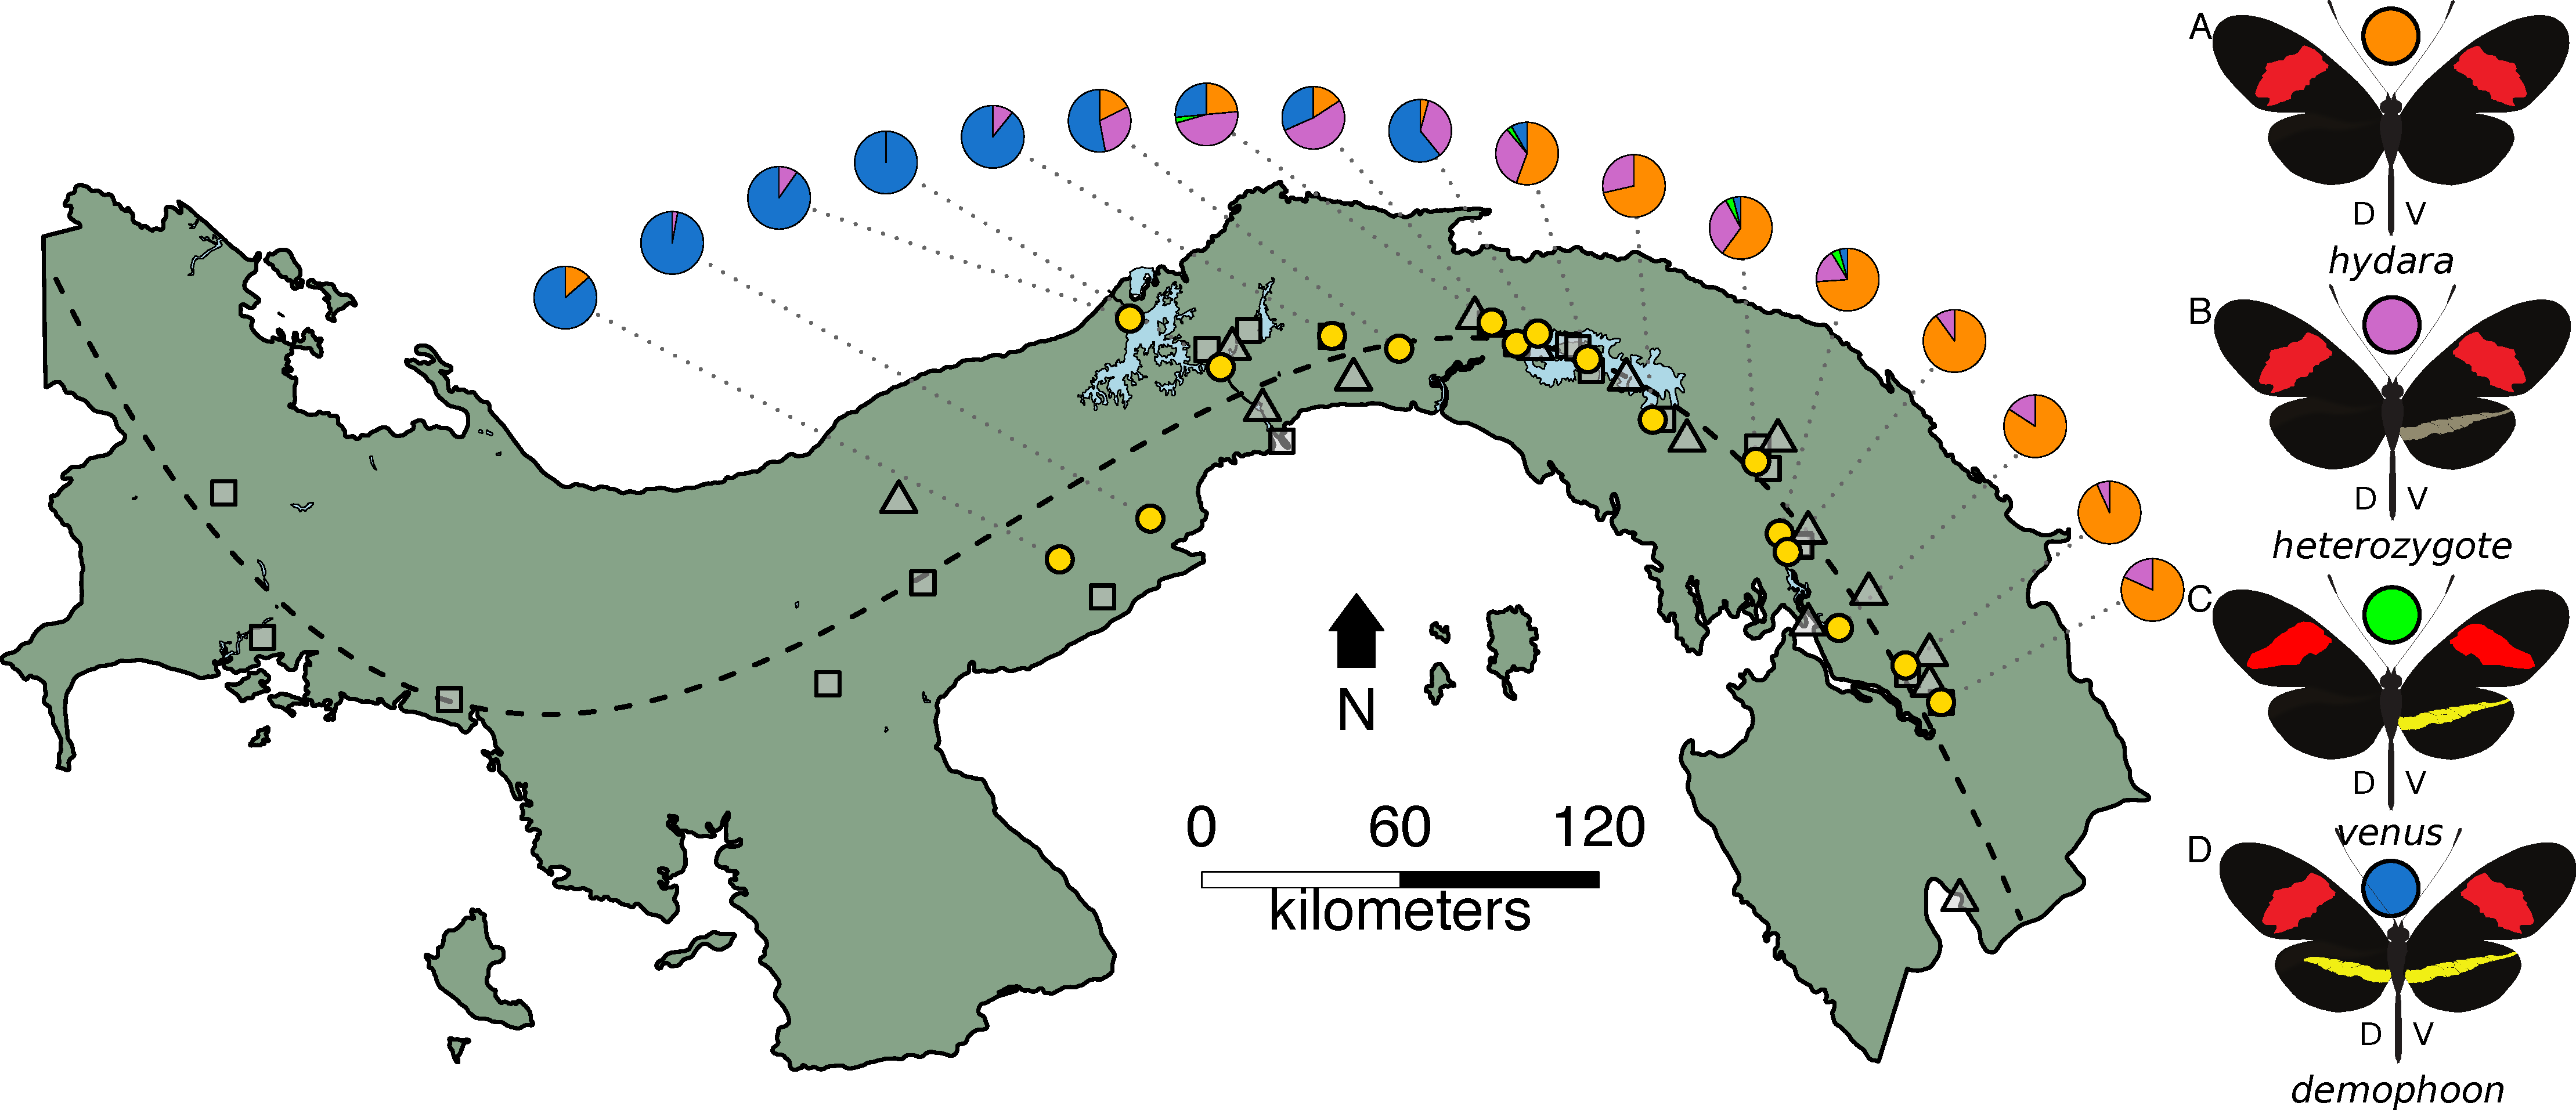
\includegraphics{figure_1_final}
\end{figure}

\pagebreak

\subsubsection{Figure 2}\label{figure-2}

\begin{figure}[h]
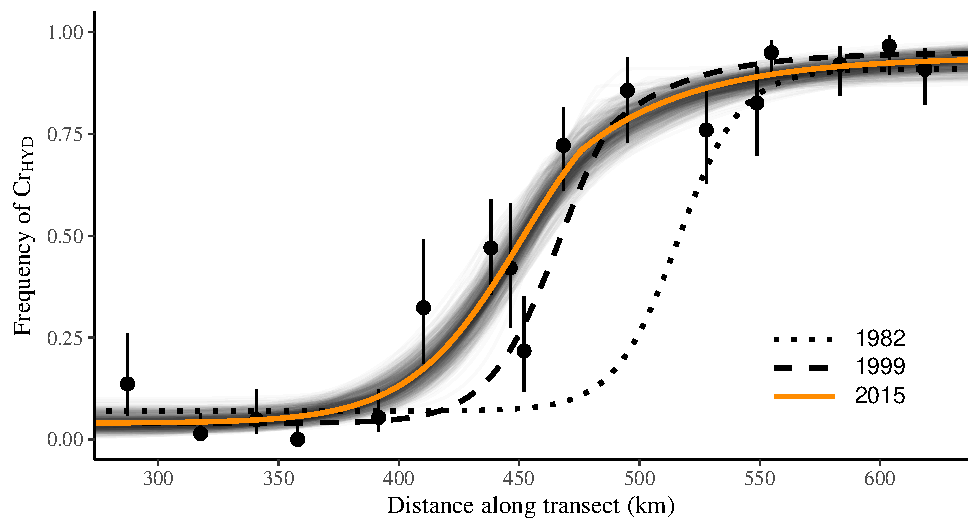
\includegraphics{figure_2}
\end{figure}

\pagebreak

\subsubsection{Figure 3}\label{figure-3}

\begin{figure}[h]
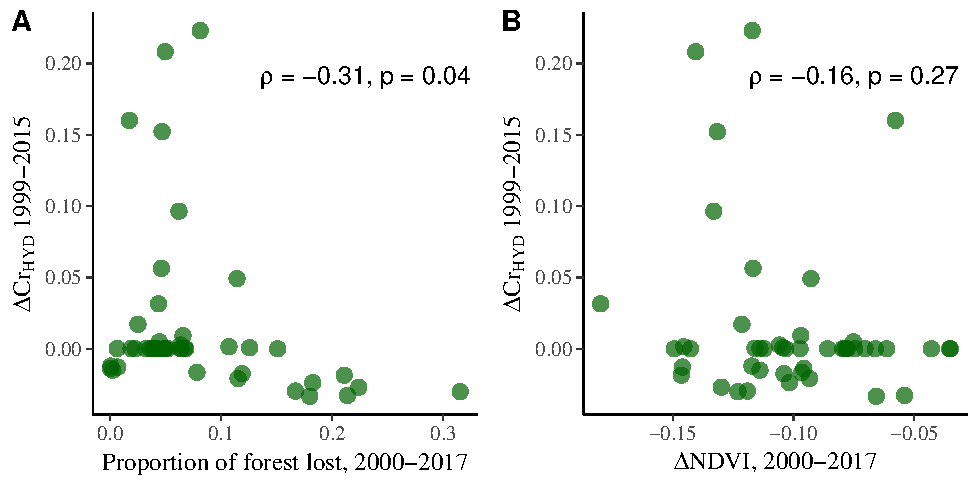
\includegraphics{figure_3}
\end{figure}

\pagebreak

\subsubsection{Table 1}\label{table-1}

\begin{table}[H]
\centering
\resizebox{\linewidth}{!}{
\begin{tabular}{clcccccc}
\toprule
\multicolumn{2}{c}{ } & \multicolumn{6}{c}{Cline parameters} \\
\cmidrule(l{3pt}r{3pt}){3-8}
\multicolumn{1}{c}{Year} & \multicolumn{1}{c}{Best model} & \multicolumn{1}{c}{center (km)} & \multicolumn{1}{c}{width (km)} & \multicolumn{1}{c}{$p_{min}$} & \multicolumn{1}{c}{$p_{max}$} & \multicolumn{1}{c}{$\delta_{R}$ (km)} & \multicolumn{1}{c}{$\tau_{R}$} \\
\cmidrule(l{3pt}r{3pt}){1-1} \cmidrule(l{3pt}r{3pt}){2-2} \cmidrule(l{3pt}r{3pt}){3-3} \cmidrule(l{3pt}r{3pt}){4-4} \cmidrule(l{3pt}r{3pt}){5-5} \cmidrule(l{3pt}r{3pt}){6-6} \cmidrule(l{3pt}r{3pt}){7-7} \cmidrule(l{3pt}r{3pt}){8-8}
1982 & no tails & 516 (511, 521) & 53 (35, 71) & 0.0684 (0.0375, 0.1009) & 0.9114 (0.8734, 0.9476) & NA & NA\\
\addlinespace
1999-2000 & right tail & 467 (462, 473) & 60 (36, 85) & 0.0376 (0.015, 0.0631) & 0.9478 (0.8976, 1) & 21 (0.0015, 53) & 0.57 (0.1758, 1)\\
\addlinespace
2015 & right tail & 451
(442, 460) & 93
(65, 123) & 0.0397
(0.01, 0.0717) & 0.9432
(0.8978, 0.9999) & 25
(5e-04, 59) & 0.6556
(0.2599, 1)\\
\bottomrule
\end{tabular}}
\end{table}


\end{document}
